In het vorige hoofdstuk is zijn de lasten van de moonrover bepaald. Op basis van deze gegevens kunnen we de juiste motor gaan selecteren voor de moonrover. Door de leverancier 'Maxon' is er een advies gedaan van een reeks motoren en transmissies;
\begin{align*}
        motor: &RE25 1187xx\\
        transmissie: &Planetary Gearhead GP xx xx
\end{align*}
In dit hoofdstuk zullen wij een keuze gaan maken voor een specifieke motor in combinatie met een specifieke transmissie.


\subsection{Motorkeuze}
Binnen de aangegeven maxon reeks hebben wij gekozen voor de RE25 118745. In theorie is het mogelijk om elke motor te kiezen binnen de aangegeven reeks in combinatie met de juiste transmissie. Voor deze specifieke situatie hebben we gekozen voor de RE25 118745. Dit is een wat kleinere motor binnen de reeks, echter is het mooie van deze motor dat hij een efficiëntie van 90\% heeft. In afbeelding \ref{fig:RE25_118745} is te zien hoe de koppel-toeren karakteristiek van de motor zich weerhoud tegen de last. In combinatie met de juiste transmissie kan deze motor goed ingezet worden bij de moonrover. In Bijlage \ref{app:datasheet motor} is de datasheet te zien van deze motor.
\begin{figure}[H]
        \centering
        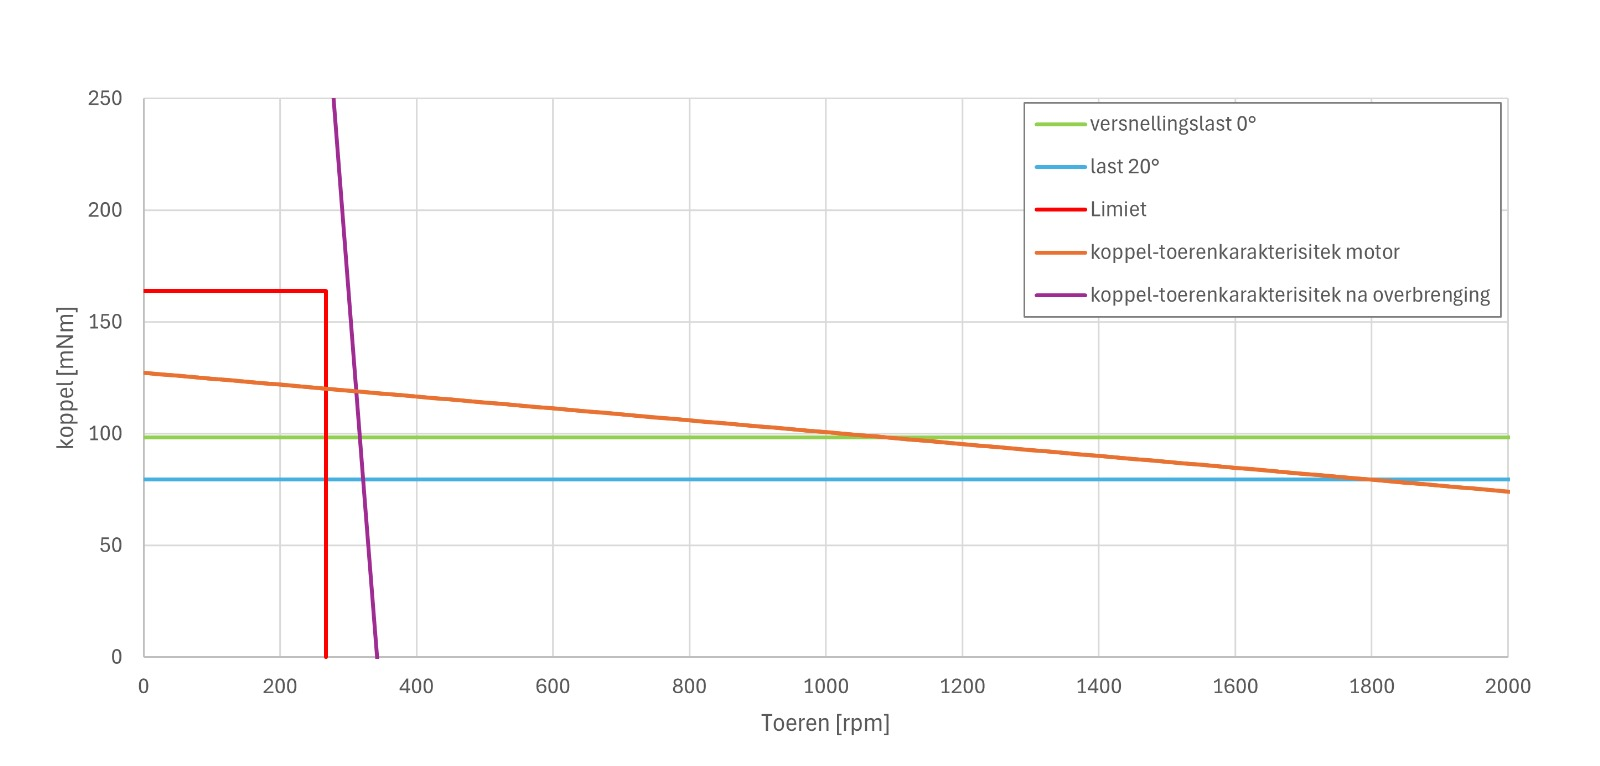
\includegraphics[scale=0.4]{nieuw.jpg}
        \caption{koppel-toeren karakteristiek met GP 32 A 166161}
        \label{fig:GP 32 A 166158}
\end{figure}

\begin{align*}
        & \text{Versnellingslast 0°} &&= \begin{aligned}[t] & \text{De hoeveelheid koppel wat nodig is om maximaal te versnellen} \\ & \text{op een helling van 0°.} \end{aligned}\\
        & \text{last 20°} &&= \begin{aligned}[t] & \text{De hoeveelheid koppel wat nodig is om stil te blijven staan} \\ & \text{op een helling van 0°.} \end{aligned}\\
        & \text{limiet} &&= \begin{aligned}[t] & \text{Dit is het limiet waarin de motor mag opereren.} \end{aligned}\\
        & \text{Koppel-toerenkarakteristiek motor} &&= \begin{aligned}[t] & \text{Dit is de koppel-toerenkarakteristiek van de motor.} \end{aligned}
    \end{align*}

\newpage

\subsection{transmissiekeuze}
In afbeelding \ref{fig:RE25_118745} is duidelijk te zien dat een transmissie aan te raden is voor het gebruiken van deze motor in de situatie van de moonrover. Het toerental van de last ligt significant lager dan het nominale toerental van de motor. Door gebruik te maken van een transmissie kunnen we er voor zorgen dat de last en de motor beter op elkaar afgestemd zullen zijn. Hierdoor zal de motor efficiënter gaan Werken omdat hij minder torque hoeft te leveren en hij vaker rond zijn nominale toerental zal draaien. In de datasheet van de  motor (bijlage \ref{app:datasheet motor}) worden er voor deze motor een aantal transmissies aangeraden binnen deze selectie en de selectie van maxon hebben wij gekozen voor de Planetary Gearhead GP 32 A 166161. Deze transmissie heeft een gear ratio van 23:1 en een efficiëntie van 75\%. Met deze eigenschappen zal de koppel-toeren karakteristiek veranderen wat te zien is in afbeelding \ref{fig:GP 32 A 166158} hier is duidelijk te zien dat met deze transmissie de wielen niet veel te hard kunnen draaien en dat er meer dan voldoende torque beschikbaar is voor de moonrover. Het extra koppeloverschot zorgt er ook nog voor dat de motor niet te hard hoeft te werken om de moonrover te kunnen verplaatsen.

        \begin{figure}[H]
                \centering
                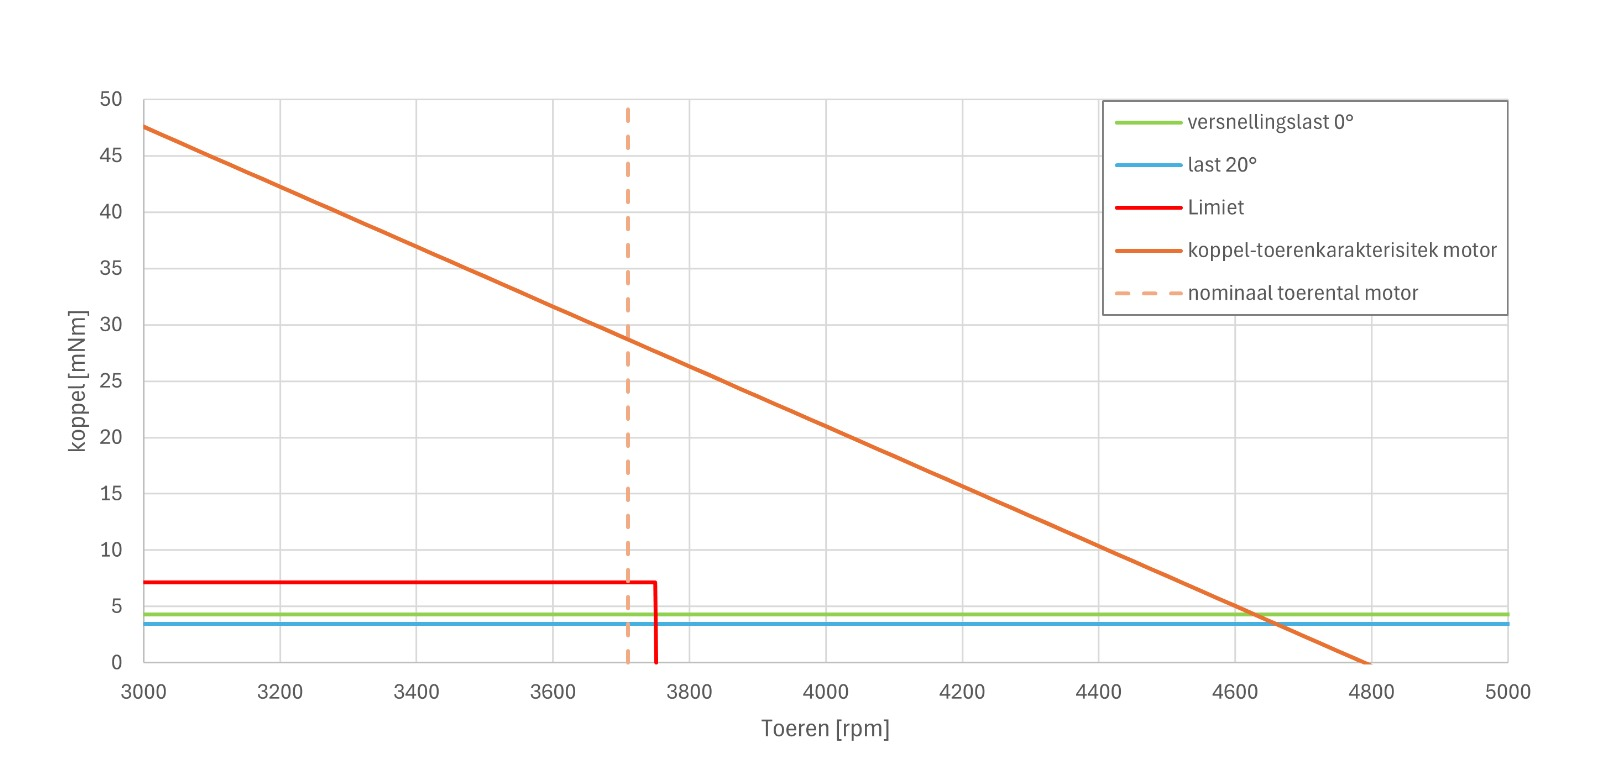
\includegraphics[scale=0.4]{overbrenging.jpg}
                \caption{koppel-toeren karakteristiek met GP 32 A 166161}
                \label{fig:GP 32 A 166158}
        \end{figure}

        \begin{align*}
                & \text{Versnellingslast 0°} &&= \begin{aligned}[t] & \text{De hoeveelheid koppel wat nodig is om maximaal te versnellen} \\ & \text{op een helling van 0°.} \end{aligned}\\
                & \text{Last 20°} &&= \begin{aligned}[t] & \text{De hoeveelheid koppel wat nodig is om stil te blijven staan} \\ & \text{op een helling van 20°.} \end{aligned}\\
                & \text{Limiet} &&= \begin{aligned}[t] & \text{Dit is de maximale koppel die geleverd mag worden om binnen}\\ & \text{zijn specificaties te blijven} \end{aligned}\\
                & \text{Koppel-toerenkarakteristiek motor} &&= \begin{aligned}[t] & \text{Dit is de koppel-toerenkarakteristiek van de motor.} \end{aligned}
            \end{align*}

\subsection{efficiëntie}

Hieronder word het vermogen berekend wat de motor opneemt bij een bepaalde hoeveelheid koppel.

\begin{multicols}{2}
        \textbf{Formules:}
        \begin{equation}
            \begin{split}
                P &= F \cdot v \\
                F &= \frac{T}{r} \\
                &\Downarrow \\
                P &= 5.25 [W]
            \end{split}
        \end{equation}

        \textbf{constante:}
        \begin{equation*}
            \begin{split}
                v &= 2.1 [m/s] \\
                T &= 0.1265[mNm]  \\
                r &= 0.075[m]
            \end{split}
        \end{equation*}
    \end{multicols}

De motor heeft een efficiëntie van een 90\%

De transmissie heeft een efficiëntie van 75\%

Samen komt dit op een totale efficiëntie van 67,5\% \\
Dit betekent dat er van het vermogen wat er in de motor gaat er 67,5\% effectief gebruikt word en de rest opgaat in warmte.

\subsection{Warmte dissipatie}

De motoren worden geleverd door het merk Maxon. Maxon heeft aangegeven dat zij de gekozen motor "maan bestendig" zullen maken. Hierbij zal ook rekening gehouden worden met de temperatuurverschillen op de maan en de warmte dissipatie hiervan. 